
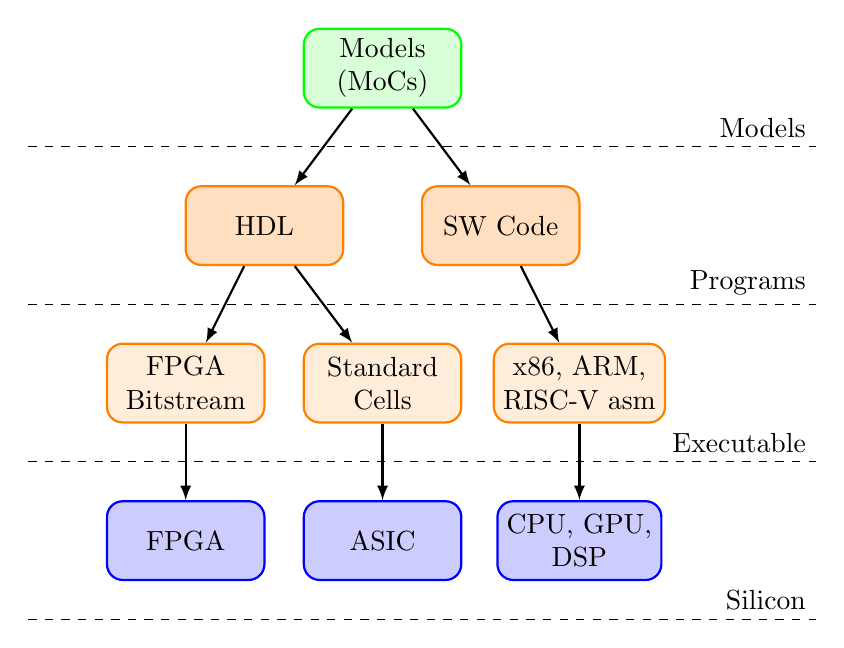
\begin{tikzpicture}{}
    \tikzstyle{every node}=[align=center];
    \tikzstyle{block} = [thick, rounded corners=2mm, draw, minimum width = 2cm, minimum height = 1cm]
    \tikzstyle{flow} = [->, thick, >= latex, rounded corners=2mm]

    \node[block, fill=green!15, draw=green] (Model) at (0.5,3) {Models \\ (MoCs)};
    \node[block, fill=orange!25, draw=orange] (VHDL) at (-1,1) {HDL};
    \node[block, fill=orange!25, draw=orange] (C) at (2,1) {SW Code};
    \node[block, fill=orange!15, draw=orange] (FPGABitstream) at (-2,-1) {FPGA \\ Bitstream};
    \node[block, fill=orange!15, draw=orange] (StandardCell) at (0.5,-1) {Standard \\ Cells};
    \node[block, fill=orange!15, draw=orange] (CPUArch) at (3,-1) {x86, ARM, \\ RISC-V asm};
    \node[block, fill=blue!20, draw=blue] (FPGA) at (-2,-3) {FPGA};
    \node[block, fill=blue!20, draw=blue] (ASIC) at (0.5,-3) {ASIC};
    \node[block, fill=blue!20, draw=blue] (CPU) at (3,-3) {CPU, GPU, \\ DSP};

    \draw[flow] (Model) -- (VHDL);
    \draw[flow] (Model) -- (C);
    \draw[flow] (VHDL) -- (FPGABitstream);
    \draw[flow] (VHDL) -- (StandardCell);
    \draw[flow] (C) -- (CPUArch);
    \draw[flow] (FPGABitstream) -- (FPGA);
    \draw[flow] (StandardCell) -- (ASIC);
    \draw[flow] (CPUArch) -- (CPU);

    %\draw [dashed] (-4,4) -- (6,4);
    \draw [dashed] (-4,0) -- (6,0) node[above left] {Programs};
    \draw [dashed] (-4,-2) -- (6,-2) node[above left] {Executable};
    \draw [dashed] (-4,2) -- (6,2) node[above left] {Models};
    \draw [dashed] (-4,-4) -- (6,-4) node[above left] {Silicon};

\end{tikzpicture}
